\beginsong{Wo ist die Kokosnuss?}[
    index={Die Affen rasen durch den Wald},
]

\beginverse
\endverse
\centering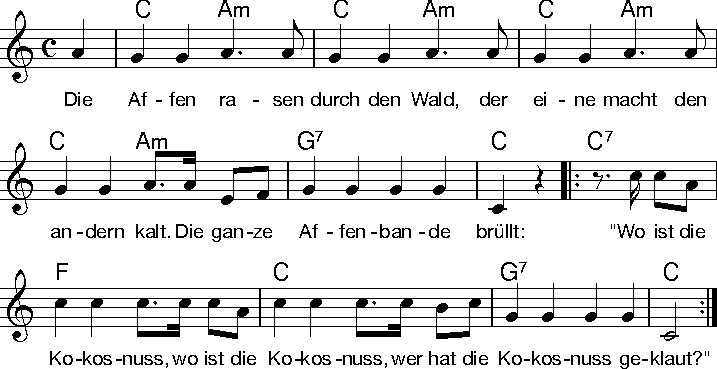
\includegraphics[width=1\textwidth]{Noten/Lied100a.pdf}

\beginverse
Die \[C]Affen\[Am]mama \[C]sitzt am \[Am]Fluss und \[C]angelt \[Am]nach der \[C]Kokos\[Am]nuss.
\endverse

\beginchorus
Die ganze \[G7]Affenbande \[C]brüllt:
\lrep '\[C7]Wo ist die \[F]Kokosnuss, wo ist die \[C]Kokosnuss,
Wer hat die \[G]Kokosnuss ge\[C]klaut?' \rrep
\endchorus

\beginverse
Der ^Affen^onkel, ^welch ein ^Grauß, reißt ^alle ^Urwald^bäume ^aus.
\endverse

\printchorus

\beginverse
Die ^Affen^tante ^kommt von ^fern, sie ^isst die ^Kokos^nuss so ^gern.
\endverse

\printchorus

\beginverse
Der ^Affen^milchmann, ^dieser ^Knilch, der ^wartet ^auf die ^Kokos^milch.
\endverse

\printchorus

\beginverse 
Das ^Affen^baby ^voll Ge^nuss hält ^in der ^Hand die ^Kokos^nuss.
\endverse

\beginchorus
Die ganze \[G]Affenbande \[C]brüllt:
\lrep '\[C7]Da ist die \[F]Kokosnuss, da ist die \[C]Kokosnuss,
Es hat die \[G]Kokosnuss ge\[C]klaut!' \rrep
\endchorus

\beginverse
Die ^Affenoma ^schreit 'Hur^ra!', die ^Kokos^nuss ist ^wieder ^da.
\endverse

\printchorus

\beginverse
Und ^die Mo^ral von ^der Ge^schicht': Klaut ^keine ^Kokos^nüsse ^nicht!
\endverse

\beginchorus
Weil sonst die \[G7]ganze Bande \[C]brüllt:
\lrep '\[C7]Wo ist die \[F]Kokosnuss, wo ist die \[C]Kokosnuss,
Wer hat die \[G7]Kokosnuss ge\[C]klaut?' \rrep
\endchorus

\endsong
